\documentclass[oneside]{book}
\usepackage{ifthen, tikz}
\usepackage{lipsum} % for generating dummy text
\usepackage{xparse}
\usepackage{amsmath}
\usepackage{amsfonts}
\usepackage{placeins}
\usepackage[T1]{fontenc}
\usepackage{import}
\usepackage{graphicx}

\usepackage{geometry}
\geometry{hmargin=4cm,vmargin=4cm}



\usetikzlibrary {arrows.meta,automata,positioning,shadows,decorations.pathmorphing, decorations.pathreplacing, decorations.shapes}
\usetikzlibrary{shapes.geometric}
\usetikzlibrary{decorations.pathreplacing}



\tikzset{%
   dot/.style={circle, inner sep=0mm, outer sep=0mm, minimum size=2mm, draw=black, fill=black},
   every loop/.style={},
}
\tikzset{
  d/.style={
    Circle[]-,
    shorten <=-2pt,
    transform canvas={shift={(-3pt, 4pt)}}
  }
}

\newcommand{\trace}[2]{% #1 is the list of items, #2 is the looseness for the loop
   %\pgfmathsetmacro{\negspace}{-1.0em - 0.5em*#2} % Calculate negative space
   \hspace{-1em}
    \begin{tikzpicture}[baseline=(node1.base), inner sep=1pt]
        % Initialize a counter for tracking the number of items
        \newcount\itemcount
        \itemcount=0
        
        % Define nodes
        \def\lastnode{node1}
        \foreach \i [count=\c] in {#1} {
            \ifnum \c=1
                \node (node\c) {$\i$}; % First node
            \else
                \node[right=1em of \lastnode] (node\c) {$\i$}; % Subsequent nodes
                \draw (\lastnode) -- (node\c); % Draw edge from last node to current
            \fi
            \global\advance\itemcount by 1
            \xdef\lastnode{node\c}
        }
        
        % Draw the loop edge
        \ifnum \itemcount=1
            \path (node1) edge [out=160, in=20, loop] ();
        \else
            \path (node1) edge [out=160, in=20, looseness=#2] (\lastnode);
        \fi
    \end{tikzpicture}
   \hspace{-1em}
}

\def\matmul#1{
   \vecmatvec{.5em}{}{#1}{}
}

\def\vecmatvec#1#2#3#4{
   \begin{tikzpicture}[baseline=-.25em, inner sep=1pt]
      \node (node0) {$#2$};
      \xdef\lastnode{node0};
      \foreach \i [count=\c] in {#3} {
         \node[right=#1 of \lastnode] (node\c) {$\i$};
         \draw (\lastnode.east) -- (node\c);
         \xdef\lastnode{node\c};
      }
      \node[right=#1 of \lastnode] (last) {$#4$};
      \draw (\lastnode.east) -- (last);
   \end{tikzpicture}
}


\def\detstack#1{
   \mathbin{\begin{tikzpicture}[baseline=(a0.base), inner sep=1pt]
      \node (a0) {#1};
      \node[right=.5em of a0] (dots) {$\cdots$};
      \node[right=.5em of dots] (a1) {#1};
      \draw (a0.north) -- ++(0,.2) coordinate (a0top);
      \draw (a1.north) -- ++(0,.2) coordinate (a1top);
      \draw (a0.south) -- ++(0,-.2) coordinate (a0bot);
      \draw (a1.south) -- ++(0,-.2) coordinate (a1bot);
      \draw[line width=2pt] (a0top -| a0.west) -- (a1top -| a1.east);
      \draw[line width=2pt] (a0bot -| a0.west) -- (a1bot -| a1.east);
   \end{tikzpicture}}
}

\newcommand{\smat}[1]{\left[\begin{smallmatrix}#1\end{smallmatrix}\right]}
\newcommand{\svec}[1]{[\begin{smallmatrix}#1\end{smallmatrix}]}
\newcommand{\E}{\mathrm{E}}
% \newcommand\sbullet[1][.5]{\mathbin{\hbox{\scalebox{#1}{$\bullet$}}}}
\newcommand\sbullet[1][1.5pt]{%
  \tikz[baseline=-0.5ex]\draw (0,0) circle (#1);%
}
\usetikzlibrary {arrows.meta}

\title{The Tensor Cookbook}
\author{Thomas Dybdahl Ahle}
\begin{document}

% Consider also taking some inspiration from https://arxiv.org/pdf/1802.01528
% "The Matrix Calculus You Need For Deep Learning"

\maketitle

\chapter{Introduction}
\paragraph{What is this?}
These pages are a guide to tensors, using the visual language of ``tensor diagrams''.
For illustrating the generality of the approach, I've tried to closely follow the legendary ``Matrix Cookbook''.
As such, most of the presentation is a collection of facts (identities, approximations, inequalities, relations, ...) about tensors and matters relating to them.
You won't find many results not in the original cookbook, but hopefully the diagrams will give you a new way to understand and appreciate them.

\paragraph{It's ongoing:}
The Matrix Cookbook is a long book, and not all the sections are equally amendable to diagrams.
Hence I've opted to skip certain sections and shorten others.
Perhaps in the future, I, or others, will expand the coverage further.

For example, while we cover all of the results on Expectation of Linear Combinations and Gaussian moments, we skip the section on general multi-variate distributions.
I have also had to rearrange the material a bit, to avoid having to introduce all the notation up front.

\paragraph{Complex Matrices and Covariance}
Tensor diagrams (or networks) are currently most often seen in Quantum Physics.
Here most values are complex numbers, which introduce some extra complexity.
In particular transposing a matrix now involves taking the conjugate (flipping the sign of the imaginary part), which introduces the need for co- and contra-variant tensors.
None of this complexity is present with standard real valued matrices, as is common e.g. in Machine Learning applications.
For simplicity I have decided to not include these complexities.

\paragraph{Tensorgrad}
The symbolic nature of tensor diagrams make the well suited for symbolic computation.

\paragraph{Advantages of Tensor Diagram Notation:}
Tensor diagram notation has many benefits compared to other notations:

Various operations, such as a trace, tensor product, or tensor contraction can be expressed simply without extra notation.
Names of indices and tensors can often be omitted. This saves time and lightens the notation, and is especially useful for internal indices which exist mainly to be summed over.
The order of the tensor resulting from a complicated network of contractions can be determined by inspection: it is just the number of unpaired lines. For example, a tensor network with all lines joined, no matter how complicated, must result in a scalar.

\tableofcontents

\section{Notation and Nomenclature}

\newenvironment{compress}{
  \renewcommand{\arraystretch}{0.6} % Set the array stretch
  \setlength{\arraycolsep}{2pt}     % Set the column separation
  \vspace{.3em}
}{
  \vspace{.3em}
  \renewcommand{\arraystretch}{1}   % Reset to default after the environment
  \setlength{\arraycolsep}{5pt}     % Reset to default column separation
}

\renewcommand{\arraystretch}{2}
\noindent
%\hspace{-1em}
\begin{tabular}[h]{lcccl}
   Dot product
   &
   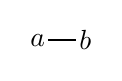
\begin{tikzpicture}[baseline=(a0.base), inner sep=1pt]
      \node (a0) {$a$};
      \node[right=1em of a0] (a1) {$b$};
      \path (a0) edge (a1);
   \end{tikzpicture}
   &
   $y=\sum_i a_i b_i$
   &
   $
\begin{compress}
\left[\begin{array}{cccc}
\cdot & \cdot & \cdot & \cdot \\
\end{array}\right]
\left[\begin{array}{c}
\cdot \\
\cdot \\
\cdot \\
\cdot \\
\end{array}\right]
\end{compress}
   $
   &
   $=y$
   \\
   Outer product
   &
   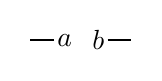
\begin{tikzpicture}[baseline=(a0.base), inner sep=1pt]
      \node (a0) {$a$};
      \node[right=.5em of a0] (a1) {$b$};
      \draw (a0.west) -- ++(-.3,0) node {};
      \draw (a1.east) -- ++(.3,0) node {};
   \end{tikzpicture}
   &
   $Y_{i,j} = a_i b_j$
   &
   $
\begin{compress}
\left[\begin{array}{c}
\cdot \\
\cdot \\
\cdot \\
\cdot \\
\end{array}\right]
\left[\begin{array}{cccc}
\cdot & \cdot & \cdot & \cdot \\
\end{array}\right]
\end{compress}
   $
   &
   $=\mathbin{
   \begin{tikzpicture}[baseline=(Y.base), inner sep=1pt]
      \node (Y) {$Y$};
      \draw (Y.east) -- ++(.3, 0);
      \draw (Y.west) -- ++(-.3, 0);
   \end{tikzpicture}}
   $
   \\
   Matrix-Vector
   &
   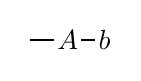
\begin{tikzpicture}[baseline=(A.base), inner sep=1pt]
      \node (A) {$A$};
      \node[right=.5em of A] (b) {$b$};
      \draw (A.west) -- ++(-.3,0) node {};
      \draw (A.east) -- (b.west);
   \end{tikzpicture}
   &
   $
   y_{i} = \sum_j A_{i,j} b_j
   $
   &
   $
   \begin{compress}
   \left[\begin{array}{cccc}
   \cdot & \cdot & \cdot & \cdot \\
   \cdot & \cdot & \cdot & \cdot \\
   \cdot & \cdot & \cdot & \cdot \\
   \cdot & \cdot & \cdot & \cdot \\
   \end{array}\right]
   \left[\begin{array}{c}
   \cdot \\
   \cdot \\
   \cdot \\
   \cdot \\
   \end{array}\right]
   \end{compress}
   $
   &
   $=\mathbin{
   \begin{tikzpicture}[baseline=(y.base), inner sep=1pt]
      \node (y) {$y$};
      \draw (y.west) -- ++(-.3, 0);
   \end{tikzpicture}
   }$
   \\
   Matrix-Matrix
   &
   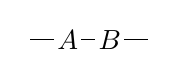
\begin{tikzpicture}[baseline=(A.base), inner sep=1pt]
      \node (A) {$A$};
      \node[right=.5em of A] (B) {$B$};
      \draw (A.west) -- ++(-.3,0) node {};
      \draw (A.east) -- (B.west);
      \draw (B.east) -- ++(.3,0) node {};
   \end{tikzpicture}
   &
   $
   Y_{i,k} = \sum_j A_{i,j} B_{j,k}
   $
   &
   $
   \begin{compress}
   \left[\begin{array}{cccc}
   \cdot & \cdot & \cdot & \cdot \\
   \cdot & \cdot & \cdot & \cdot \\
   \cdot & \cdot & \cdot & \cdot \\
   \cdot & \cdot & \cdot & \cdot \\
   \end{array}\right]
   \left[\begin{array}{cccc}
   \cdot & \cdot & \cdot & \cdot \\
   \cdot & \cdot & \cdot & \cdot \\
   \cdot & \cdot & \cdot & \cdot \\
   \cdot & \cdot & \cdot & \cdot \\
   \end{array}\right]
   \end{compress}
   $
   &
   $=\mathbin{
   \begin{tikzpicture}[baseline=(Y.base), inner sep=1pt]
      \node (Y) {$Y$};
      \draw (Y.west) -- ++(-.3, 0);
      \draw (Y.east) -- ++(.3, 0);
   \end{tikzpicture}
   }$
\end{tabular}

The rank-4 copy tensor, $C_{i,j,k,l} = [i=j=k=l]$,

\begin{tikzpicture}[baseline=(a0.base), inner sep=0pt]
   \node (a0) {$\sbullet$};
   \draw (a0) -- ++(.17,.17);
   \draw (a0) -- ++(.17,-.17);
   \draw (a0) -- ++(-.17,.17);
   \draw (a0) -- ++(-.17,-.17);
\end{tikzpicture},
differs from the outer product of two identity matrices (in the Cookbook denoted $J$),
which satisfies $J_{i,j,k,l} = [i=k][j=l]$ and which we'd write as
$J=\vcenter{\hbox{
   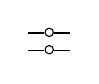
\begin{tikzpicture}[inner sep=0pt]
   \node (a0) {$\sbullet$};
   \draw (a0.east) -- ++(.2,0);
   \draw (a0.west) -- ++(-.2,0);
   \node[below=.2em of a0] (a1) {$\sbullet$};
   \draw (a1.east) -- ++(.2,0);
   \draw (a1.west) -- ++(-.2,0);
\end{tikzpicture}}}$,
and satisfies, for example, $\frac{dX}{dX}=J$.

\section{Basics}

\begin{tikzpicture}[baseline=(A.base), inner sep=1pt]
   \node (A) {$A$};
   \draw (A.west) -- ++(-.3, 0);
   \draw (A.east) -- ++(+.3, 0);
\end{tikzpicture}
=
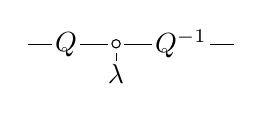
\begin{tikzpicture}[baseline=(Q.base), inner sep=1pt]
   \node (Q) {$Q$};
   \draw (Q.west) -- ++(-.3, 0);
   \node[right=1em of Q] (dot) {$\sbullet$};
   \path (Q) edge (dot);
   \node[below=.3em of dot] (e) {$\lambda$};
   \path (dot) edge (e);
   \node[right=1em of dot] (Qi) {$Q^{-1}$};
   \path (dot) edge (Qi);
   \draw (Qi.east) -- ++(.3, 0);
\end{tikzpicture}
where $\lambda_i$ is the $i$th eigenvalue of $A$.

More general principles:
\begin{enumerate}
   \item You can contract edges in any order.
   \item You can always contract connected subgraphs of Copy tensors.
   \item distributive law of sums/products.
   \item Sums and broadcasting.
\end{enumerate}

%\begin{figure}[h]
%\centering{
%\resizebox{75mm}{!}{\input{figures/path1.pdf_tex}}
%\caption{Top view.}
%\label{fig:topView}
%}
%\end{figure}

\begin{figure}[h]
\centering{
\def\svgwidth{.5\linewidth}
\import{figures/}{path1.pdf_tex}
\caption{Contract spiders}
\label{fig:spiders}
}
\end{figure}


\begin{figure}[h]
\centering{
\def\svgwidth{.75\linewidth}
\import{figures/}{path2.pdf_tex}
\caption{Eliminate Identity}
\label{fig:identity}
}
\end{figure}


\begin{figure}[h]
\centering{
\def\svgwidth{\linewidth}
\import{figures/}{path3.pdf_tex}
\caption{Distributive law}
\label{fig:dist}
}
\end{figure}
\subsection{Trace}

The ``trace'' of a square matrix is defined $\mathrm{Tr}(A) = \sum_i A_{i,i}$.
In tensor diagram notation, that corresponds to a self-edge: $\trace{A}{1}$.

\begin{align*}
   \sum_{i=1}^{n} A_{ii} &= \mathrm{Tr}(A) = \mathrm{Tr}(A I)
   &
   \trace{A}{1} &= \trace{A, \sbullet}{2}
   \tag{11}
   \\%%%%%%%%%%%%%%%%%%%%%%%%%%%%%%%%%%%%%%%%
   \mathrm{Tr}(A) &= \sum_i \lambda_i = \langle 1, \lambda\rangle
   &
   \trace{A}1 &=
   \hspace{-2em}
   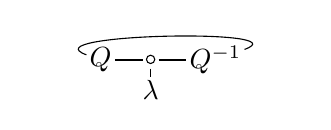
\begin{tikzpicture}[baseline=(Q.base), inner sep=1pt]
      \node (Q) {$Q$};
      \node[right=1em of Q] (dot) {$\sbullet$};
      \path (Q) edge (dot);
      \node[below=.3em of dot] (e) {$\lambda$};
      \path (dot) edge (e);
      \node[right=1em of dot] (Qi) {$Q^{-1}$};
      \path (dot) edge (Qi);
      \path (Q) edge [out=160, in=20, looseness=1] (Qi);
   \end{tikzpicture}
   \hspace{-2em}
   \tag{12}
   \\%%%%%%%%%%%%%%%%%%%%%%%%%%%%%%%%%%%%%%%%
   \mathrm{Tr}(A) &= \mathrm{Tr}(A^T)
   &
   \trace{A}1 &= \trace{A}1
   \tag{13}
   \\%%%%%%%%%%%%%%%%%%%%%%%%%%%%%%%%%%%%%%%%
   \mathrm{Tr}(AB) &= \mathrm{Tr}(BA)
   &
   \trace{A,B}2 &= \trace{B,A}2
   \tag{14}
   \\%%%%%%%%%%%%%%%%%%%%%%%%%%%%%%%%%%%%%%%%
   \tag{15}
   \mathrm{Tr}(A+B)
   &= \mathrm{Tr}(A) + \mathrm{Tr}(B)
   &
   \trace{(A+B),\sbullet}1
   %\trace{(\matmul{A}+\matmul{B}),\sbullet}{2}
   &= \trace{A,\sbullet}2
 \\&&&+\trace{B,\sbullet}2
   \\%%%%%%%%%%%%%%%%%%%%%%%%%%%%%%%%%%%%%%%%
   \tag{16}
   \mathrm{Tr}(ABC) &= \mathrm{Tr}(BCA)
   &
   \trace{A,B,C}1 &= \trace{B,C,A}1
   \\
                  & = \mathrm{Tr}(CAB)
                  &&= \trace{C,A,B}1
   \\[0.5em]
   %%%%%%%%%%%%%%%%%%%%%%%%%%%%%%%%%%%%%%%%
   \tag{17}
   a^T a &= \mathrm{Tr}(a a^T)
   &
   \vecmatvec{1em}{a}{}{a}
   &=
   \mathrm{Tr}(
   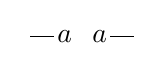
\begin{tikzpicture}[baseline=(a0.base), inner sep=1pt]
      \node (a0) {$a$};
      \node[right=.5em of a0] (a1) {$a$};
      \draw (a0.west) -- ++(-.3,0) node {};
      \draw (a1.east) -- ++(.3,0) node {};
   \end{tikzpicture}
   )
 \\&&&=
   \hspace{-1em}
   
\begin{tikzpicture}[baseline=(a0.base), inner sep=1pt]
      \node (a0) {$a$};
      \node[right=1em of a0] (a1) {$a$};
      \path (a0) edge [out=160, in=20, looseness=2] (a1);
   \end{tikzpicture}
   \hspace{-1em}
\end{align*}


\chapter{Simple Derivatives}

\section{Derivatives of Matrices, Vectors and Scalar Forms}

\subsection{First Order}

The Matrix Cookbook defines the single-entry matrix $J^{i,j} \in R^{n\times n}$ as the matrix which is zero everywhere except in the entry $(i, j)$ in which it is 1.
Alternatively we could write $J^{i,j}_{n,m} = [i=n][j=m]$.

\begin{align*}
   \tag{69}
   \frac{\partial x^T a}{\partial x}
   &= \frac{\partial a^T x}{\partial x}
   = a
   &
      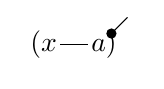
\begin{tikzpicture}[baseline=(a0.base), inner sep=1pt]
         \node (a0) {$(x$};
         \node[right=1em of a0] (a1) {$a)$};
         \path (a0) edge (a1);
         \draw [d] (a1.east) -- ++(.2,.2);
      \end{tikzpicture}
   &=
      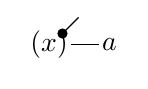
\begin{tikzpicture}[baseline=(a0.base), inner sep=1pt]
         \node (a0) {$(x)$};
         \node[right=1em of a0] (a1) {$a$};
         \path (a0) edge (a1);
         \draw [d] (a0.east) -- ++(.2,.2);
      \end{tikzpicture}
   =
      \begin{tikzpicture}[baseline=(a0.base), inner sep=1pt]
         \node (a0) {};
         \node[right=1em of a0] (a1) {$a$};
         \path (a0) edge (a1);
         \draw (a0.east) -- ++(-.1,-.2);
      \end{tikzpicture}
   \\
   %%%%%%%%%%%%%%%%%%%%%%%%%%%%%%%%%%%%%%%%
   \tag{70}
   \frac{\partial a^T X b}{\partial X} &= ab^T
   &
      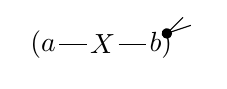
\begin{tikzpicture}[baseline=(a0.base), inner sep=1pt]
         \node (a0) {$(a$};
         \node[right=1em of a0] (a1) {$X$};
         \node[right=1em of a1] (a2) {$b)$};
         \path (a0) edge (a1);
         \path (a1) edge (a2);
         \draw[d] (a2.east) -- ++(.2,.2);
         \draw[d] (a2.east) -- ++(.3,.1);
      \end{tikzpicture}
   &=
      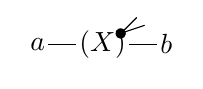
\begin{tikzpicture}[baseline=(a0.base), inner sep=1pt]
         \node (a0) {$a$};
         \node[right=1em of a0] (a1) {$(X)$};
         \node[right=1em of a1] (a2) {$b$};
         \path (a0) edge (a1);
         \path (a1) edge (a2);
         \draw[d] (a1.east) -- ++(.2,.2);
         \draw[d] (a1.east) -- ++(.3,.1);
      \end{tikzpicture}
      =
      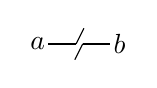
\begin{tikzpicture}[baseline=(a0.base), inner sep=1pt]
         \node (a0) {$a$};
         \node[right=1em of a0] (a1) {};
         \node[right=1em of a1] (a2) {$b$};
         \path (a0) edge (a1);
         \path (a1) edge (a2);
         \draw (a1.west) -- ++(.1,.2);
         \draw (a1.east) -- ++(-.1,-.2);
      \end{tikzpicture}
   \\
   %%%%%%%%%%%%%%%%%%%%%%%%%%%%%%%%%%%%%%%%
   \tag{73}
   \frac{\partial X}{\partial X_{i,j}} &= J^{i,j}
   &
      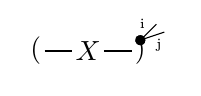
\begin{tikzpicture}[baseline=(a0.base), inner sep=1pt]
         \node (a0) {$($};
         \node[right=1em of a0] (a1) {$X$};
         \node[right=1em of a1] (a2) {$)$};
         \path (a0) edge (a1);
         \path (a1) edge (a2);
         \draw[d] (a2.east) -- ++(.2,.2) node[midway, above left, font=\tiny] {i};
         \draw[d] (a2.east) -- ++(.3,.1) node[midway, below right, font=\tiny] {j};
      \end{tikzpicture}
   &=
      \begin{tikzpicture}[baseline=(a0.base), inner sep=1pt]
         \node (a0) {};
         \node[right=1em of a0] (a1) {};
         \node[right=1em of a1] (a2) {};
         \path (a0) edge (a1);
         \path (a1) edge (a2);
         \draw (a1.west) -- ++(.1,.2) node[midway, above left, font=\tiny] {i};
         \draw (a1.east) -- ++(-.1,-.2) node[midway, below right, font=\tiny] {j};
      \end{tikzpicture}
   \\
   %%%%%%%%%%%%%%%%%%%%%%%%%%%%%%%%%%%%%%%%
   \tag{74}
   \frac{\partial (X A)_{i,j}}{\partial X_{m,n}} &= (J^{m,n} A)_{i,j}
   &
      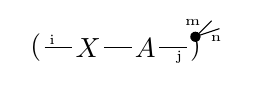
\begin{tikzpicture}[baseline=(a0.base), inner sep=1pt]
         \node (a0) {$($};
         \node[right=1em of a0] (a1) {$X$};
         \node[right=1em of a1] (a2) {$A$};
         \node[right=1em of a2] (a3) {$)$};
         \draw (a0) -- (a1) node[midway, above left, font=\tiny] {i};
         \draw (a1) -- (a2);
         \draw (a2) -- (a3) node[midway, below right, font=\tiny] {j};
         \draw[d] (a3.east) -- ++(.2,.2) node[midway, above left, font=\tiny] {m};
         \draw[d] (a3.east) -- ++(.3,.1) node[midway, below right, font=\tiny] {n};
      \end{tikzpicture}
   &=
      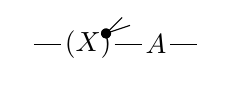
\begin{tikzpicture}[baseline=(a0.base), inner sep=1pt]
         \node (a0) {};
         \node[right=1em of a0] (a1) {$(X)$};
         \node[right=1em of a1] (a2) {$A$};
         \node[right=1em of a2] (a3) {};
         \path (a0) edge (a1);
         \path (a1) edge (a2);
         \path (a2) edge (a3);
         \draw[d] (a1.east) -- ++(.2,.2);
         \draw[d] (a1.east) -- ++(.3,.1);
      \end{tikzpicture}
 \\&&&=
      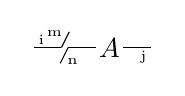
\begin{tikzpicture}[baseline=(a0.base), inner sep=1pt]
         \node (a0) {};
         \node[right=1em of a0] (a1) {};
         \node[right=1em of a1] (a2) {$A$};
         \node[right=1em of a2] (a3) {};
         \draw (a0) -- (a1) node[midway, above left, font=\tiny] {i};
         \draw (a1) -- (a2);
         \draw (a2) -- (a3) node[midway, below right, font=\tiny] {j};
         \draw (a1.west) -- ++(.1,.2) node[midway, above left, font=\tiny] {m};
         \draw (a1.east) -- ++(-.1,-.2) node[midway, below right, font=\tiny] {n};
      \end{tikzpicture}
\end{align*}

\subsection{Second Order}
\noindent
\makebox[\textwidth]{\parbox{1.1\textwidth}{%
\begin{align*}
   \tag{76}
   \frac{\partial}{\partial X_{i,j}}
   \sum_{k,l,m,n} X_{k,l} X_{m,n}
   &= (\sum_{k,l} X_{k,l})^2
   %&= \frac{\partial \|X\|_F^2}{\partial X_{i,j}}
   %&= 2\, \sum_{k,l} X_{k,l}
   &
   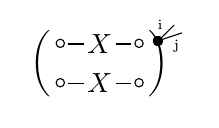
\begin{tikzpicture}[baseline=.5em, inner sep=1pt]
      \node (a0) at (0,0) {$\sbullet$};
      \node (a1) at (.5,0) {$X$};
      \node (a2) at (1,0) {$\sbullet$};
      \path (a0) edge (a1);
      \path (a1) edge (a2);
      \node (b0) at (0, .5) {$\sbullet$};
      \node (b1) at (.5, .5) {$X$};
      \node (b2) at (1, .5) {$\sbullet$};
      \path (b0) edge (b1);
      \path (b1) edge (b2);
      \node at (-.25, .25) {$\bigg($};
      \node at (1.25, .25) {$\bigg)$};
      \draw[d] (1.35, .4) -- ++(.2,.2) node[midway, above left, font=\tiny] {i};
      \draw[d] (1.35, .4) -- ++(.3,.1) node[midway, below right, font=\tiny] {j};
   \end{tikzpicture}
   &=
   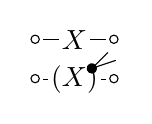
\begin{tikzpicture}[baseline=.5em, inner sep=1pt]
      \node (a0) at (0,0) {$\sbullet$};
      \node (a1) at (.5,0) {$(X)$};
      \node (a2) at (1,0) {$\sbullet$};
      \path (a0) edge (a1);
      \path (a1) edge (a2);
      \node (b0) at (0, .5) {$\sbullet$};
      \node (b1) at (.5, .5) {$X$};
      \node (b2) at (1, .5) {$\sbullet$};
      \path (b0) edge (b1);
      \path (b1) edge (b2);
      \draw[d] (.83,.0) -- ++(.2,.2);
      \draw[d] (.83,.0) -- ++(.3,.1);
   \end{tikzpicture}
   +
   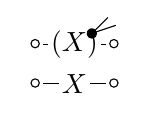
\begin{tikzpicture}[baseline=.5em, inner sep=1pt]
      \node (a0) at (0,0) {$\sbullet$};
      \node (a1) at (.5,0) {$X$};
      \node (a2) at (1,0) {$\sbullet$};
      \path (a0) edge (a1);
      \path (a1) edge (a2);
      \node (b0) at (0, .5) {$\sbullet$};
      \node (b1) at (.5, .5) {$(X)$};
      \node (b2) at (1, .5) {$\sbullet$};
      \path (b0) edge (b1);
      \path (b1) edge (b2);
      \draw[d] (0.83,.5) -- ++(.2,.2);
      \draw[d] (0.83,.5) -- ++(.3,.1);
   \end{tikzpicture}
   %\\[.3em]
   \\
   &= 2\, \sum_{k,l} X_{k,l}
   &&=
   2\,
   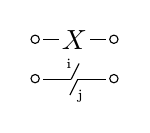
\begin{tikzpicture}[baseline=.5em, inner sep=1pt]
      \node (a0) at (0,0) {$\sbullet$};
      \node (a1) at (.5,0) {};
      \node (a2) at (1,0) {$\sbullet$};
      \path (a0) edge (a1);
      \path (a1) edge (a2);
      \node (b0) at (0, .5) {$\sbullet$};
      \node (b1) at (.5, .5) {$X$};
      \node (b2) at (1, .5) {$\sbullet$};
      \path (b0) edge (b1);
      \path (b1) edge (b2);
      \draw (a1.west) -- ++(.1,.2) node[midway, above left, font=\tiny] {i};
      \draw (a1.east) -- ++(-.1,-.2) node[midway, below right, font=\tiny] {j};
   \end{tikzpicture}
   %%%%%%%%%%%%%%%%%%%%%%%%%%%%%%%%%%%%%%%%
   \\[.5em]
   \tag{77} 
   \frac{\partial b^T X^T X c}{\partial X} &= X(bc^T + cb^T) 
   &
   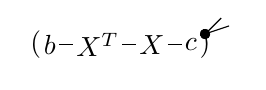
\begin{tikzpicture}[baseline=(a0.base), inner sep=1pt]
      \node (a0) {$(\vecmatvec{.5em}{b}{X^T,X}{c})$};
      \draw[d] (a0.east) -- ++(.2,.2);
      \draw[d] (a0.east) -- ++(.3,.1);
   \end{tikzpicture}
   &=
   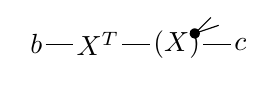
\begin{tikzpicture}[baseline=(a0.base), inner sep=1pt]
      \node (a0) {$b$};
      \node[right=1em of a0] (a1) {$X^T$};
      \node[right=1em of a1] (a2) {$(X)$};
      \node[right=1em of a2] (a3) {$c$};
      \draw (a0) -- (a1);
      \draw (a1) -- (a2);
      \draw (a2) -- (a3);
      \draw[d] (a2.east) -- ++(.2,.2);
      \draw[d] (a2.east) -- ++(.3,.1);
   \end{tikzpicture}
 \\&&&+
   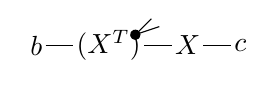
\begin{tikzpicture}[baseline=(a0.base), inner sep=1pt]
      \node (a0) {$b$};
      \node[right=1em of a0] (a1) {$(X^T)$};
      \node[right=1em of a1] (a2) {$X$};
      \node[right=1em of a2] (a3) {$c$};
      \draw (a0) -- (a1);
      \draw (a1) -- (a2);
      \draw (a2) -- (a3);
      \draw[d] (a1.east) -- ++(.2,.2);
      \draw[d] (a1.east) -- ++(.3,.1);
   \end{tikzpicture}
   \\[.3em]&&&=
   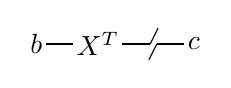
\begin{tikzpicture}[baseline=(a0.base), inner sep=1pt]
      \node (a0) {$b$};
      \node[right=1em of a0] (a1) {$X^T$};
      \node[right=1em of a1] (a2) {};
      \node[right=1em of a2] (a3) {$c$};
      \draw (a0) -- (a1);
      \draw (a1) -- (a2);
      \draw (a2) -- (a3);
      \draw (a2.west) -- ++(.1,.2);
      \draw (a2.east) -- ++(-.1,-.2);
   \end{tikzpicture}
 \\&&&+
   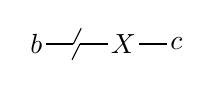
\begin{tikzpicture}[baseline=(a0.base), inner sep=1pt]
      \node (a0) {$b$};
      \node[right=1em of a0] (a1) {};
      \node[right=1em of a1] (a2) {$X$};
      \node[right=1em of a2] (a3) {$c$};
      \draw (a0) -- (a1);
      \draw (a1) -- (a2);
      \draw (a2) -- (a3);
      \draw (a1.west) -- ++(.1,.2);
      \draw (a1.east) -- ++(-.1,-.2);
   \end{tikzpicture}
   \\[.3em]&&&=
   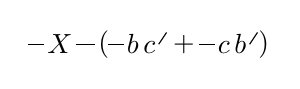
\begin{tikzpicture}[baseline=(a0.base), inner sep=1pt]
      \node (a0) {$X$};
      \node[right=.7em of a0] (a1) {$($};
      \node[right=.4em of a1] (a2) {$b\, c$};
      \node[right=.4em of a2] (a4) {$+$};
      \node[right=.6em of a4] (a5) {$c\, b$};
      \node[right=.2em of a5] (a7) {$)$};
      \draw (a0.west) -- ++(-.2,0);
      \draw (a0) -- (a1);
      \draw (a2.west) -- ++(-.2,0);
      \draw (a2.east) -- ++(.1,.15);
      \draw (a5.west) -- ++(-.2,0);
      \draw (a5.east) -- ++(.1,.15);
   \end{tikzpicture}
   \\
   \tag{78} 
   \frac{\partial}{\partial x} (Bx+b)^T C (Dx+d) &= B^TC(Dx+d)&&
                                \\&+D^TC^T(Bx+b) 
   &
   \dots &
   \\
   \tag{79} 
   \frac{\partial}{\partial X_{i,j}} (X^TBX)_{k,l} &= \delta_{l,j}(X^TB)_{k,i}
   %  \\&+ \delta_{k,j}(BX)_{i,l} 
   &
   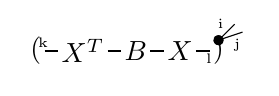
\begin{tikzpicture}[baseline=(a0.base), inner sep=1pt]
      \node (a0) {$($};
      \node[right=.5em of a0] (a1) {$X^T$};
      \node[right=.5em of a1] (a2) {$B$};
      \node[right=.5em of a2] (a3) {$X$};
      \node[right=.5em of a3] (a4) {$)$};
      \draw (a0) -- (a1) node[midway, above left, font=\tiny] {k};
      \draw (a1) -- (a2);
      \draw (a2) -- (a3);
      \draw (a3) -- (a4) node[midway, below right, font=\tiny] {l};
      \draw[d] (a4.east) -- ++(.2,.2) node[midway, above left, font=\tiny] {i};
      \draw[d] (a4.east) -- ++(.3,.1) node[midway, below right, font=\tiny] {j};
   \end{tikzpicture}
   &=
   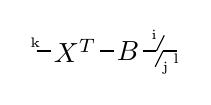
\begin{tikzpicture}[baseline=(a0.base), inner sep=1pt]
      \node (a0) {};
      \node[right=.5em of a0] (a1) {$X^T$};
      \node[right=.5em of a1] (a2) {$B$};
      \node[right=.5em of a2] (a3) {};
      \node[right=.5em of a3] (a4) {};
      \draw (a0) -- (a1) node[midway, above left, font=\tiny] {k};
      \draw (a1) -- (a2);
      \draw (a2) -- (a3);
      \draw (a3) -- (a4) node[midway, below right, font=\tiny] {l};
      \draw (a3.west) -- ++(.1,.2) node[midway, above left, font=\tiny] {i};
      \draw (a3.east) -- ++(-.1,-.2) node[midway, below right, font=\tiny] {j};
   \end{tikzpicture}
   \\
   &+ \delta_{k,j}(BX)_{i,l}
   &&+
   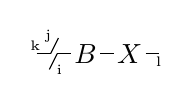
\begin{tikzpicture}[baseline=(a0.base), inner sep=1pt]
      \node (a0) {};
      \node[right=.5em of a0] (a1) {};
      \node[right=.5em of a1] (a2) {$B$};
      \node[right=.5em of a2] (a3) {$X$};
      \node[right=.5em of a3] (a4) {};
      \draw (a0) -- (a1) node[midway, above left, font=\tiny] {k};
      \draw (a1) -- (a2);
      \draw (a2) -- (a3);
      \draw (a3) -- (a4) node[midway, below right, font=\tiny] {l};
      \draw (a1.west) -- ++(.1,.2) node[midway, above left, font=\tiny] {j};
      \draw (a1.east) -- ++(-.1,-.2) node[midway, below right, font=\tiny] {i};
   \end{tikzpicture}
   %%%%%%%%%%%%%%%%%%%%%%%%%%%%%%%%%%%%%%%%
   \\
   \tag{80} 
   \frac{\partial}{\partial X_{i,j}} X^TBX &= X^TBJ^{i,j} + J^{j,i}BX 
   &
   \dots &
   %%%%%%%%%%%%%%%%%%%%%%%%%%%%%%%%%%%%%%%%
   \\
   \tag{81} 
   \frac{\partial}{\partial x} x^TBx &= (B+B^T)x 
   &
   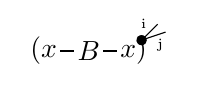
\begin{tikzpicture}[baseline=(a0.base), inner sep=1pt]
      \node (a0) {$(x$};
      \node[right=.5em of a0] (a1) {$B$};
      \node[right=.5em of a1] (a2) {$x)$};
      \draw (a0) -- (a1);
      \draw (a1) -- (a2);
      \draw[d] (a2.east) -- ++(.2,.2) node[midway, above left, font=\tiny] {i};
      \draw[d] (a2.east) -- ++(.3,.1) node[midway, below right, font=\tiny] {j};
   \end{tikzpicture}
   &=
   \vecmatvec{.5em}{}{B}{x}
   + \vecmatvec{.5em}{x}{B}{}
 \\&&&=
   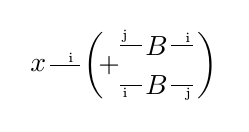
\begin{tikzpicture}[baseline=.5em, inner sep=1pt]
      \node (a0) at (0,0) {};
      \node (a1) at (.5,0) {$B$};
      \node (a2) at (1,0) {};
      \draw (a0) -- (a1) node[midway, below left, font=\tiny] {i};
      \draw (a1) -- (a2) node[midway, below right, font=\tiny] {j};
      \node (b0) at (0, .5) {};
      \node (b1) at (.5, .5) {$B$};
      \node (b2) at (1, .5) {};
      \draw (b0) -- (b1) node[midway, above left, font=\tiny] {j};
      \draw (b1) -- (b2) node[midway, above right, font=\tiny] {i};
      \node (l) at (-.3, .25) {$\bigg($};
      \node at (1.15, .25) {$\bigg)$};
      \node at (-.1, .25) {$+$};
      \node (x) at (-1,.25) {$x$};
      \draw (x) -- (l) node[midway, above right, font=\tiny] {i};
   \end{tikzpicture}
   %%%%%%%%%%%%%%%%%%%%%%%%%%%%%%%%%%%%%%%%
   \\
   \tag{82} 
   \frac{\partial}{\partial X} b^T X^T D X c &= D^T X b c^T + DXcb^T 
   &
   \dots &
   \\
   \tag{83} 
   \frac{\partial}{\partial X} (Xb+c)^T D (Xb+c) &= (D+D^T)(Xb+c)b^T 
   &
   \dots &
   \\
\end{align*}
}}

Assume $W$ is symmetric, then... (84) - (88)

\subsection{Higher-order and non-linear}
...

\subsection{Gradient and Hessian}
...
\section{Derivatives of Traces}
Assume F(X) to be a differentiable function of each of the elements of X. It
then holds that
\[\frac{d \mathrm{Tr}(F(x))}{dX} = f(X)^T,\]
where $f(\cdot)$ is the scalar derivative of $F(\cdot)$.

TODO: To show this with tensor diagrams, we first need to introduce our notation for functions.

% Many more examples here: https://mbustamanter.github.io/ssg-blog/matder1/

\subsection{First Order}

\begin{tabular}[h]{lcc}
   (99) &
   $ \frac{\partial}{\partial X} \mathrm{Tr}(X) = I $
   &
   $ (\trace{X}{1}) = \trace{(X)}{0} = \trace{\phantom{X}}2 = \matmul{\sbullet} $
   \\
   (100) &
   $ \frac{\partial}{\partial X} \mathrm{Tr}(XA) = A^T $
   &
   $ (\trace{X,A}{2}) = \trace{(X), A}{2} = \trace{\phantom{X}, A}2 = \matmul{A^T} $
   \\
   (101) &
   $ \frac{\partial}{\partial X} \mathrm{Tr}(AXB) = A^TB^T $
   &
   $ (\trace{A,X,B}{2}) = \trace{A, (X), B}{2} = \matmul{A^T, B^T} $
   \\
\end{tabular}
Continues for (102-105).
The last one uses the Kronecker product, which we may have to introduce first.

\subsection{Second Order}

\subsection{Higher Order}

\subsection{Other}



\chapter{Statistics and Probability}
\subsection{Definition of Moments}
Let $x\in\mathbb R^{n}$ is a random variable.
We write $m = E[x]\in\mathbb R^n$ for the expectation and
$M=\mathrm{Var}[x] = E[(x-m)(x-m)^T]$ for the covariance (when these quantities are defined.)

In tensor diagrams, we will use square brackets:
\[
\mathbin{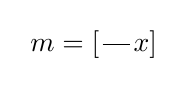
\begin{tikzpicture}[baseline=(n0.base), inner sep=1pt]
   \node (n0) at (0,0) {$m=[$};
   \node [right=1em of n0] (n1) {$x]$};
   \draw (n0) -- (n1);
\end{tikzpicture}}
\quad\text{and}\quad
\mathbin{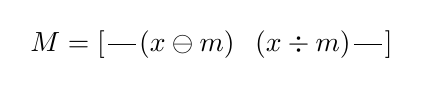
\begin{tikzpicture}[baseline=(n0.base), inner sep=1pt]
   \node (n0) at (0,0) {$M=[$};
   \node [right=1em of n0] (n1) {$(x\ominus m)$};
   \node [right=.5em of n1] (n2) {$(x\div m)$};
   \node [right=1em of n2] (n3) {$]$};
   \draw (n0) -- (n1);
   \draw (n2) -- (n3);
\end{tikzpicture}}
\]
Note we used the German minus, $\div$, to distinguish subtraction from contraction edges.

We can also define the third and fourth centralized moment tensors
\[
   M_3=
   \renewcommand*{\arraystretch}{1.3}
   \begin{bmatrix}
      \vecmatvec{1em}{(x\div m)}{}{} \\
      \vecmatvec{1em}{(x\div m)}{}{} \\
      \vecmatvec{1em}{(x\div m)}{}{}
   \end{bmatrix}
\quad\text{and}\quad
M_4=
   \renewcommand*{\arraystretch}{1.3}
   \begin{bmatrix}
      \vecmatvec{1em}{(x\div m)}{}{} \\
      \vecmatvec{1em}{(x\div m)}{}{} \\
      \vecmatvec{1em}{(x\div m)}{}{} \\
      \vecmatvec{1em}{(x\div m)}{}{}
   \end{bmatrix}
.
\]

\subsection{Expectation of Linear Combinations}
General principle: The ``linearity of expectation'' lets you pull out all parts of the graph not involving $X$.

\subsubsection{Linear Forms}
\begin{align*}
   \tag{312}
   \E[AXB+C] &= A \E[X] B + C
   &
   \renewcommand*{\arraystretch}{1.3}
   \begin{bmatrix}
      \matmul{A,X,B} \\+\, \matmul{C}
   \end{bmatrix}
   &=
   \renewcommand*{\arraystretch}{1.3}
   \begin{matrix}
      \matmul{A,[X],B} \\+\, \matmul{C}
   \end{matrix}
   %%%%%%%%%%%%%%%%%%%%%%%%%%%%%%%%%%%%%%%%
   \\
   \tag{313}
   \mathrm{Var}[Ax] &= A \mathrm{Var}[x] A^T
   &
   \renewcommand*{\arraystretch}{1.3}
   \begin{bmatrix}
      \vecmatvec{.5em}{A}{}{x} \div [\vecmatvec{.5em}{A}{}{x}] \\
      \vecmatvec{.5em}{A}{}{x} \div [\vecmatvec{.5em}{A}{}{x}]
   \end{bmatrix}
   &=
   \renewcommand*{\arraystretch}{1.3}
   \begin{bmatrix}
      \vecmatvec{.5em}{A}{}{(x\div m)} \\
      \vecmatvec{.5em}{A}{}{(x\div m)}
   \end{bmatrix}
 \\&&&=
   \vcenter{\hbox{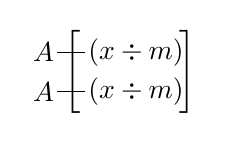
\begin{tikzpicture}[inner sep=1pt]
      \node (n1) at (0,-.25) {$\vecmatvec{1em}{A}{}{(x\div m)}$};
      \node (n2) at (0,.25) {$\vecmatvec{1em}{A}{}{(x\div m)}$};
      \node at (-.45, 0) {$\Bigg[$};
      \node at (1, 0) {$\Bigg]$};
   \end{tikzpicture}}}
 \\&&& =
   \vecmatvec{.5em}{}{A,M_2,A}{}
\end{align*}

\subsubsection{Quadratic Forms}
\begin{align*}
   \E[x^T A x] &= \mathrm{Tr}(A \Sigma) + \mu^T A \mu
   \\
   [\vecmatvec{.5em}{x}{A}{x}]
   &=
   [\vecmatvec{.5em}{(x\div \mu)}{A}{(x \div\mu)}
   +
   \vecmatvec{.5em}{\mu}{A}{\mu}]
   \\
   &=
   \mathbin{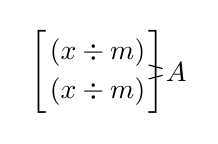
\begin{tikzpicture}[inner sep=1pt]
      \node (n1) at (0,-.25) {$(x\div m)$};
      \node (n2) at (0,.25) {$(x\div m)$};
      \node at (-.75, 0) {$\Bigg[$};
      \node at (.75, 0) {$\Bigg]$};
      \node (A) at (1, 0) {$A$};
      \draw (n1) -- (A);
      \draw (n2) -- (A);
   \end{tikzpicture}}
   +
   \vecmatvec{.5em}{\mu}{A}{\mu}
   \\
   &=
   \trace{\Sigma,A}2
   +
   \vecmatvec{.5em}{\mu}{A}{\mu}
\end{align*}

\subsubsection{Cubic Forms}

\subsection{Weighted Scalar Variable}
Let $y=w^T x$, and let $m=E[y]$, then
\begin{align*}
   \E[y] &= m = w^T \mu
   \\
   \E[(y-m)^2] &= \vecmatvec{.5em}{w}{M_2}{w}
   \\
   \E[(y-m)^3] &=
   \mathbin{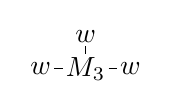
\begin{tikzpicture}[baseline=(a0.base), inner sep=1pt]
      \node (a0) {$M_3$};
      \node[above=.3em of a0] (n0) {$w$};
      \node[right=.3em of a0] (n1) {$w$};
      \node[left=.3em of a0] (n3) {$w$};
      \draw (a0.north) -- (n0);
      \draw (a0.east) -- (n1);
      \draw (a0.west) -- (n3);
   \end{tikzpicture}}
   \\
   \E[(y-m)^4] &=
   \mathbin{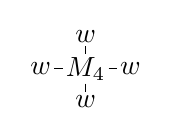
\begin{tikzpicture}[baseline=(a0.base), inner sep=1pt]
      \node (a0) {$M_4$};
      \node[above=.3em of a0] (n0) {$w$};
      \node[right=.3em of a0] (n1) {$w$};
      \node[below=.3em of a0] (n2) {$w$};
      \node[left=.3em of a0] (n3) {$w$};
      \draw (a0.north) -- (n0);
      \draw (a0.east) -- (n1);
      \draw (a0.south) -- (n2);
      \draw (a0.west) -- (n3);
   \end{tikzpicture}}
\end{align*}
For specific distributions, like $x$ Gaussian, we can often reduce the moment tensors further.
Khintchine's inequality also gives a way to bound all of these in terms of $E[(y-m)^2]$.


\subsection{Gaussian Moments}
\subsubsection{Mean and covariance of linear forms}
\subsubsection{Mean and variance of square forms}
\subsubsection{Cubic forms}
\subsubsection{Mean of Quartic Forms}
\subsubsection{Gaussian Integration by Parts}
General principle for Gaussian expectations.



\chapter{Solutions and Decompositions}


\section{Kronecker and Vec Operator}

The Kronecker Product and Vec Operator are ways to avoid dealing with tensors, and generally best avoided.


\tikzstyle{triangle}=[
    regular polygon,
    regular polygon sides=3,
    rotate=270,
    scale=.5,
    draw
]

\begin{tikzpicture}[baseline=-.5em]
\node (X) at (1,0) {X};
\node (A) at (2,1) {A};
\node (B) at (2,-1) {B};
\node[triangle] (c1) at (3,0) {};
\node (c2) at (4,0) {};
\draw (X) -- (A);
\draw (X) -- (B);
\draw (A) -- (c1);
\draw (B) -- (c1);
\draw (c1) edge[double] (c2);
\draw [decorate,decoration={brace,amplitude=5pt,mirror,raise=4ex}]
  (.5,-.75) -- (3.5,-.75) node[midway,yshift=-3em]{$\mathrm{vec}(A^T X B)$};
\end{tikzpicture}
=
\begin{tikzpicture}[baseline=-.5em]
\node (X) at (.5,0) {X};
\node[triangle] (c0) at (1.5,0) {};
\node[triangle, rotate=180] (c1) at (2.5,0) {};
\node (A) at (3.5,1) {A};
\node (B) at (3.5,-1) {B};
\node[triangle] (c2) at (4.5,0) {};
\node (c3) at (5.5,0) {};
\draw (X) edge[bend left] (c0);
\draw (X) edge[bend right] (c0);
\draw[double] (c0) -- (c1);
\draw (c1) -- (A) -- (c2);
\draw (c1) -- (B) -- (c2);
\draw[double] (c2) -- (c3);
\draw [decorate,decoration={brace,amplitude=5pt,mirror,raise=4ex}]
  (.5,-.75) -- (3.5,-.75) node[midway,yshift=-3em]{$\mathrm{vec}(X)^T(A \otimes B)$};
\end{tikzpicture}
\\
Some basic properties:
\\
\begin{tikzpicture}[baseline=-.5em]
\node (a0) at (.5,1) {};
\node (a1) at (.5,-1) {};
\node[triangle] (c0) at (1.5,0) {};
\node (a2) at (2.5,0) {};
\draw (a0) -- (c0) node[midway, above right, font=\tiny] {i};
\draw (a1) -- (c0) node[midway, above left, font=\tiny] {j};
\draw (c0) -- (a2) node[midway, above, font=\tiny] {k};
\end{tikzpicture}
= [i + j n = k]
\\
Opposing triangles cancel:
\\
\begin{tikzpicture}[baseline=-.3em]
\node (X) at (.5,0) {\phantom{X}};
\node[triangle] (c0) at (1.5,0) {};
\node[triangle, rotate=180] (c1) at (2.5,0) {};
\node (Y) at (3.5,0) {\phantom{Y}};
\draw (X) edge[bend left] (c0);
\draw (X) edge[bend right] (c0);
\draw[double] (c0) -- (c1);
\draw (Y) edge[bend left] (c1);
\draw (Y) edge[bend right] (c1);
\end{tikzpicture}
=
\begin{tikzpicture}[baseline=-.3em]
\node (X) at (0,0) {\phantom{X}};
\node (Y) at (1.5,0) {\phantom{Y}};
\draw (X) edge[bend left] (Y);
\draw (X) edge[bend right] (Y);
\end{tikzpicture}
\\and\\
\begin{tikzpicture}[baseline=-.3em]
\node (X) at (.5,0) {\phantom{X}};
\node[triangle, rotate=180] (c0) at (1.5,0) {};
\node[triangle] (c1) at (2.5,0) {};
\node (Y) at (3.5,0) {\phantom{Y}};
\draw[double] (X) -- (c0);
\draw (c0) edge[bend left] (c1);
\draw (c0) edge[bend right] (c1);
\draw[double] (Y) -- (c1);
\end{tikzpicture}
=
\begin{tikzpicture}[baseline=-.3em]
\node (X) at (0,0) {\phantom{X}};
\node (Y) at (1.5,0) {\phantom{Y}};
\draw[double] (X) -- (Y);
\end{tikzpicture}



\subsubsection{The Kronecker Product}
The Kronecker product of an $m\times n$ matrix $A$ and an $r \times q$ matrix $B$, is an $mr \times nq$ matrix, $A \otimes B$ defined as
\[
   A \otimes B = \begin{bmatrix}
      A_{1,1} B & A_{1,2} B & \cdots & A_{1,n} B \\
      A_{2,1} B & A_{2,2} B & \cdots & A_{2,n} B \\
      \vdots & \vdots & \ddots & \vdots \\
      A_{m,1} B & A_{m,2} B & \cdots & A_{m,n} B
   \end{bmatrix}
\]

The Kronecker product has the following properties:
\begin{align}
   A \otimes (B + C) &= A \otimes B + A \otimes C \\
   A \otimes (B \otimes C) &= (A \otimes B) \otimes C \\
   a A \otimes b B &= a b (A \otimes B) \\
   (A \otimes B)^T &= A^T \otimes B^T \\
   (A \otimes B)(C \otimes D) &= AC \otimes BD \\
   (A \otimes B)^{-1} &= A^{-1} \otimes B^{-1} \\
   \mathrm{Tr}(A \otimes B) &= \mathrm{Tr}(A) \mathrm{Tr}(B)
\end{align}

\subsubsection{The Vec Operator}
A few more good properties here.

\begin{align}
   \mathrm{vec}(AXB) &= (B^T \otimes A)\mathrm{vec}(X) \\
   \mathrm{Tr}(A^TB) &= \mathrm{vec}(A)^T \mathrm{vec}(B) \\
   \mathrm{vec}(A + B) &= \mathrm{vec}(A) +  \mathrm{vec}(B) \\
   \mathrm{vec}(a A) &= a \mathrm{vec}(A) \\
   a^T X B X^T c &= \mathrm{vec}(X)^T (B\otimes ca^T) \mathrm{vec}(X)
\end{align}


\section{Solutions to linear equations}
\subsection{The Lyapunov Equation}
This is a nice trick that can be well explained.
Though it requires some talk about Kronecker products.
Also ``(5.1.11) Encapsulating Sum'' which is a generalization.

\section{Eigenvalues and Eigenvectors}

\section{Decompositions}
\subsection{Singular Value Decomposition}
\subsection{Triangular Decomposition}
\subsection{LDM Decomposition}
\subsection{LDL Decomposition}




\chapter{Determinant and Inverses}

\section{Determinant}

It's convenient to write the determinant in tensor notation as
\[\mathrm{det}(A)=
\frac{1}{n!}\,\mathbin{
\begin{tikzpicture}[baseline=(a0.base), inner sep=1pt]
   \node (a0) {$A$};
   \node[right=.5em of a0] (dots) {$\cdots$};
   \node[right=.5em of dots] (a1) {$A$};
   \draw (a0.north) -- ++(0,.2) coordinate (a0top);
   \draw (a1.north) -- ++(0,.2) coordinate (a1top);
   \draw (a0.south) -- ++(0,-.2) coordinate (a0bot);
   \draw (a1.south) -- ++(0,-.2) coordinate (a1bot);
   \draw[line width=2pt] (a0top -| a0.west) -- (a1top -| a1.east);
   \draw[line width=2pt] (a0bot -| a0.west) -- (a1bot -| a1.east);
\end{tikzpicture}}
\]
where
$\mathbin{
\begin{tikzpicture}[baseline=(a0.south)-3em, inner sep=1pt]
   \node (a0) {\tiny $i_1$};
   \node[right=.5em of a0] (a1) {\tiny $i_2$};
   \node[right=.5em of a1] (dots) {$\dots$};
   \node[right=.5em of dots] (a2) {\tiny $i_n$};
   \draw (a0.south) -- ++(0,-.25) coordinate (a0bot);
   \draw (a1.south) -- ++(0,-.25) coordinate (a1bot);
   \draw (a2.south) -- ++(0,-.25) coordinate (a2bot);
   \draw[line width=2pt] (a0bot -| a0.west) -- (a2bot -| a2.east);
\end{tikzpicture}}
=\varepsilon_{i_1,\dots,i_n}$
is the rank-$n$ Levi-Civita tensor defined by
\[
   \varepsilon_{i_1, \dots, i_n} =
   \begin{cases}
      \mathrm{sign}(\sigma) & \sigma=(i_1, \dots, i_n) \text{ is a permutation} \\
      0 & \text{otherwise.}
   \end{cases}
\]
To see that the definition makes sense, let's first consider
\begin{align*}
   \mathrm{det}(I)=
   \frac{1}{n!}
\mathbin{
   \begin{tikzpicture}[baseline=(dots.base), inner sep=1pt]
      \node (a0) {};
      \node[right=.5em of a0] (a1) {};
      \node[right=.5em of a1] (dots) {$\dots$};
      \node[right=.5em of dots] (a2) {};
      \draw (a0.south) -- ++(0,.3) coordinate (a0top);
      \draw (a1.south) -- ++(0,.3) coordinate (a1top);
      \draw (a2.south) -- ++(0,.3) coordinate (a2top);
      \draw (a0.north) -- ++(0,-.3) coordinate (a0bot);
      \draw (a1.north) -- ++(0,-.3) coordinate (a1bot);
      \draw (a2.north) -- ++(0,-.3) coordinate (a2bot);
      \draw[line width=2pt] (a0top -| a0.west) -- (a2top -| a2.east);
      \draw[line width=2pt] (a0bot -| a0.west) -- (a2bot -| a2.east);
   \end{tikzpicture}
}
%&
=
\frac{1}{n!}
\sum_{i_1, \dots, i_n, j_1, \dots, j_n}
   \varepsilon_{i_1, \dots, i_n}
   \varepsilon_{j_1, \dots, j_n}
   [i=j]
%\\&
=
   \frac{1}{n!}
   \sum_{i_1, \dots, i_n}
   \varepsilon_{i_1, \dots, i_n}^2
%\\&
%=
%   \sum_{i_1, \dots, i_n}
%   [(i_1, \dots, i_n)\text{ is a permutation}]
%\\&
= 1.
\end{align*}
In general we get from the permutation definition of the determinant:
\begin{align*}
   \detstack{A}
   &=
   \sum_{i_1, \dots, i_n, j_1, \dots, j_n}
   \varepsilon_{i_1, \dots, i_n}
   \varepsilon_{j_1, \dots, j_n}
   A_{i_1,j_1} \cdots A_{i_n,j_n}
   \\&=
   \sum_{\sigma, \tau}
   \mathrm{sign}(\sigma)
   \mathrm{sign}(\tau)
   A_{\sigma_1,\tau_1} \cdots A_{\sigma_n,\tau_n}
   \\&=
   \sum_{\sigma}
   \mathrm{sign}(\sigma)
   \sum_\tau
   \mathrm{sign}(\tau)
   A_{\sigma_1,\tau_1} \cdots A_{\sigma_n,\tau_n}
   \\&=
   \sum_{\sigma}
   \mathrm{sign}(\sigma)^2
   \mathrm{det}(A)
   \\&=
   n! \mathrm{det}(A).
\end{align*}
The definition generalizes to Cayley's ``hyper determinants'' by $\dots$.

A curious property is that
\[
   \mathbin{\begin{tikzpicture}[baseline=(a0.base), inner sep=1pt]
      \node (a0) {$A$};
      \node[right=.5em of a0] (dots) {$\cdots$};
      \node[right=.5em of dots] (a1) {$A$};
      \draw (a0.north) -- ++(0,.2) coordinate (a0top);
      \draw (a1.north) -- ++(0,.2) coordinate (a1top);
      \draw (a0.south) -- ++(0,-.2) coordinate (a0bot);
      \draw (a1.south) -- ++(0,-.2) coordinate (a1bot);
      \draw[line width=2pt] (a0bot -| a0.west) -- (a1bot -| a1.east);
   \end{tikzpicture}}
   =
   \mathbin{\begin{tikzpicture}[baseline=(a0.base), inner sep=1pt]
      \node (a0) {$A$};
      \node[right=.5em of a0] (dots) {$\cdots$};
      \node[right=.5em of dots] (a1) {$A$};
      \draw (a0.north) -- ++(0,.2) coordinate (a0top);
      \draw (a1.north) -- ++(0,.2) coordinate (a1top);
      \draw (a0.south) -- ++(0,-.2) coordinate (a0bot);
      \draw (a1.south) -- ++(0,-.2) coordinate (a1bot);
      \draw[line width=2pt] (a0top -| a0.west) -- (a1top -| a1.east);
      \draw[line width=2pt] (a0bot -| a0.west) -- (a1bot -| a1.east);
      \node[above=1.5em of a0] (b0) {$\phantom{A}$};
      \node[above=1.5em of dots] (d1) {$\cdots$};
      \node[above=1.5em of a1] (b1) {$\phantom{A}$};
      \draw (b0.south) -- ++(0,-.2) coordinate (b0bot);
      \draw (b1.south) -- ++(0,-.2) coordinate (b1bot);
      \draw[line width=2pt] (b0bot -| b0.west) -- (b1bot -| b1.east);
   \end{tikzpicture}}
\]

\renewcommand{\arraystretch}{2}
\begin{tabular}[h]{lcc}
   (18) &
   $ \mathrm{det}(A) = \prod_i \lambda_i $
   &
   \dots
   \\
   (19) &
   $ \mathrm{det}(cA) = c^n \mathrm{det}(A) $
   &
   $ \detstack{$cA$} = c^n \detstack{$A$} $
   \\
   (20) &
   $ \mathrm{det}(A) = \mathrm{det}(A^T) $
   &
   \dots
   \\
   (21) &
   $ \mathrm{det}(AB) = \mathrm{det}(A)\mathrm{det}(B) $
   &
   $
   \mathbin{\begin{tikzpicture}[baseline=(a0.base), inner sep=1pt]
      \node (a0) {$B$};
      \node[right=.5em of a0] (dots) {$\cdots$};
      \node[right=.5em of dots] (a1) {$B$};
      \draw (a0.south) -- ++(0,-.2) coordinate (a0bot);
      \draw (a1.south) -- ++(0,-.2) coordinate (a1bot);
      \node[above=.5em of a0] (b0) {$A$};
      \node[above=.5em of dots] (d1) {$\cdots$};
      \node[above=.5em of a1] (b1) {$A$};
      \draw (b0.south) -- (a0.north);
      \draw (b1.south) -- (a1.north);
      \draw (b0.north) -- ++(0,.2) coordinate (b0top);
      \draw (b1.north) -- ++(0,.2) coordinate (b1top);
      \draw[line width=2pt] (b0top -| b0.west) -- (b1top -| b1.east);
      \draw[line width=2pt] (a0bot -| a0.west) -- (a1bot -| a1.east);
   \end{tikzpicture}}
   =
   \mathbin{\begin{tikzpicture}[baseline=(a0.base), inner sep=1pt]
      \node (a0) {$B$};
      \node[right=.5em of a0] (dots) {$\cdots$};
      \node[right=.5em of dots] (a1) {$B$};
      \draw (a0.north) -- ++(0,.2) coordinate (a0top);
      \draw (a1.north) -- ++(0,.2) coordinate (a1top);
      \draw (a0.south) -- ++(0,-.2) coordinate (a0bot);
      \draw (a1.south) -- ++(0,-.2) coordinate (a1bot);
      \draw[line width=2pt] (a0top -| a0.west) -- (a1top -| a1.east);
      \draw[line width=2pt] (a0bot -| a0.west) -- (a1bot -| a1.east);
      \node[above=1.5em of a0] (b0) {$A$};
      \node[above=1.5em of dots] (d1) {$\cdots$};
      \node[above=1.5em of a1] (b1) {$A$};
      \draw (b0.north) -- ++(0,.2) coordinate (b0top);
      \draw (b1.north) -- ++(0,.2) coordinate (b1top);
      \draw (b0.south) -- ++(0,-.2) coordinate (b0bot);
      \draw (b1.south) -- ++(0,-.2) coordinate (b1bot);
      \draw[line width=2pt] (b0top -| b0.west) -- (b1top -| b1.east);
      \draw[line width=2pt] (b0bot -| b0.west) -- (b1bot -| b1.east);
   \end{tikzpicture}}
   $
   \\
   (22) &
   $ \mathrm{det}(A^{-1}) = 1/\mathrm{det}(A) $
   &
   \dots
   \\
   (23) &
   $ \mathrm{det}(A^n) = \mathrm{det}(A)^n $
   &
   \dots
   \\
   (24) &
   $ \mathrm{det}(I+uv^T) = 1 + u^Tv $
   &
   \dots
   \\
\end{tabular}


\section{Inverses}
Might be reduced, unless cofactor matrices have a nice representation?


\chapter{Functions}
Stuff about analytical matrix functions.
Such as Exponential Matrix Function.
I'd rather talk about my general function notation.
And maybe about taylor series?

\subsection{Pseudo-linear form}
Maybe this should just be an example in a table?

Derivation of Peyman Milanfar's gradient
\begin{align*}
\mathrm{d}[\mathbf{f}(\mathbf{x})] & =\mathrm{d}[\mathbf{A}(\mathbf{x}) \mathbf{x}] \\
& =\mathrm{d}[\mathbf{A}(\mathbf{x})] \mathbf{x}+\mathbf{A}(\mathbf{x}) \mathrm{d} \mathbf{x} \\
& =\operatorname{vec}\{\mathrm{d}[\mathbf{A}(\mathbf{x})] \mathbf{x}\}+\mathbf{A}(\mathbf{x}) \mathrm{d} \mathbf{x} \\
& =\operatorname{vec}\{\mathbf{I} \mathrm{d}[\mathbf{A}(\mathbf{x})] \mathbf{x}\}+\mathbf{A}(\mathbf{x}) \mathrm{d} \mathbf{x} \\
& =\left(\mathbf{x}^T \otimes \mathbf{I}\right) \operatorname{vec}\{\mathrm{d}[\mathbf{A}(\mathbf{x})]\}+\mathbf{A}(\mathbf{x}) \mathrm{d} \mathbf{x} \\
& =\left(\mathbf{x}^T \otimes \mathbf{I}\right) \mathrm{D} \operatorname{vec}[\mathbf{A}(\mathbf{x})] \mathrm{d} \mathbf{x}+\mathbf{A}(\mathbf{x}) \mathrm{d} \mathbf{x} \\
& =\left[\left(\mathbf{x}^T \otimes \mathbf{I}\right) \mathrm{D} \operatorname{vec}[\mathbf{A}(\mathbf{x})]+\mathbf{A}(\mathbf{x})\right] \mathrm{d} \mathbf{x}
\end{align*}



\section{Taylor Series}
I've always wanted to write these out properly with tensors.

\chapter{Advanced Derivatives}

\section{Derivatives of vector norms}

\subsection{Two-norm}
\begin{align}
   \frac{d}{dx}\|x-a\|_2 &= \frac{x-a}{\|x-a\|_2}
   \\
   \frac{d}{dx}\frac{x-a}{\|x-a\|_2} &= \frac{I}{\|x-a\|_2} - \frac{(x-a)(x-a)^T}{\|x-a\|_2^3}
   \\
   \frac{d}{dx}\|x\|_2^2 = \frac{d}{dx}\|x^T x\|_2 = 2x
\end{align}

\section{Derivatives of matrix norms}

\section{Derivatives of Structured Matrices}
\subsection{The Chain Rule}
Sometimes the objective is to find the derivative of a matrix which is a function of another matrix.

\subsection{The Hessian Chain Rule}
See main.tex

\subsection{Symmetric}
\subsection{Diagonal}
\subsection{Toeplitz}

\section{Derivatives of a Determinant}
\section{General forms}
\section{Linear forms}
\section{Square forms}


\section{Derivatives of an Inverse}
\section{Derivatives of Eigenvalues}


\chapter{Special Matrices}
\subsection{Block matrices}
Stuff like Schur complements is interesting.
But can we say anything useful using tensor diagrams?

\subsection{The Discrete Fourier Transform Matrix}
I think FFT can be nicely described with diagrams

Let's start with the Hadamard matrix:
$H_n = \smat{1 & 1 \\ 1 & -1}^{\otimes n}$.
Hm. It's just a bunch of matrices below each other, kinda boring.

What about the FFT?
Does that require a bit more?

\subsection{Hermitian Matrices and skew-Hermitian}
Complex. Skip
\subsection{Idempotent Matrices}
Skip
\subsection{Orthogonal matrices}
Skip
\subsection{Positive Definite and Semi-definite Matrices}
Skip
\subsection{Singleentry Matrix, The}
Describes the matrix $J$.
All of this is trivial with diagrams.
\subsection{Symmetric, Skew-symmetric/Antisymmetric}
Could introduce Penrose's symmetric tensors here?
\subsection{Toeplitz Matrices}
Could talk about the convolution tensor here...
\subsection{Units, Permutation and Shift}
Not that interesting...
\subsection{Vandermonde Matrices}
Does this have a nice description?
Not a lot of properties are given in the Cookbook.



\chapter{Machine Learning Applications}

\section{Least Squares}

\section{Hessian of Cross Entropy Loss}

\section{Convolutional Neural Networks}

\section{Transformers / Attention}

\section{Tensor Sketch}

\chapter{Tensorgrad}

Implementation details

\section{Simplification Rules}
\section{Functions}
\section{Isomorphisms}

\chapter{Appendix}
Contains some proofs, such as of equation 524 or 571.
They are pretty long and could be useful for contrasting with the diagram proofs.

\end{document}
